\documentclass[a4paper,12pt]{article}
\usepackage[slovene]{babel}
\usepackage[utf8]{inputenc}
\usepackage[T1]{fontenc}
\usepackage{lmodern}
\usepackage{amsmath,amsfonts}
\usepackage{enumitem}
\usepackage{graphicx}
\usepackage{subfigure}
\usepackage{mathtools}
\usepackage{xcolor}
\usepackage{url}
\pagenumbering{roman}

\begin{document}

\newcommand{\N}{\mathbb{N}}
\newcommand{\R}{\mathbb{R}}
\newcommand\sbullet[1][.5]{\mathbin{\vcenter{\hbox{\scalebox{#1}{$\bullet$}}}}}
%\theoremstyle{definition} % tekst napisan pokoncno
\newtheorem{definicija}{Definicija}[section]
\newtheorem{primer}[definicija]{Primer}
\newtheorem{opomba}[definicija]{Opomba}

\title{Diskretne Coonsove ploskve}
\author{Matej Rojec, Vito Rozman}
\date{\today}

\maketitle

\newpage

\tableofcontents
\listoffigures

\newpage

\section{Uvod}

V seminarski nalogi bomo obravnavali ploskve, ki interpolirajo štiri mejne krivulje,
ki so definirane vsaka na svoji stranici pravokotnika $[0,1]^2$. 
Te ploskve bomo imenovali diskretne Coonsove ploskve, 
ki jih bomo določili z bilinearno interpolacijo kontrolnih točk.
Potem si bomo ogledali posplošitev
Coonsovih ploskev na stalne ploskve, ki jih bomo dobili 
z reševanjem linearnega sistema enačb. Pogledali si bomo tudi problem, ko imamo namesto štirih mejnih 
krivulj podane samo tri robne krivulje, ki so definirane nad trikotnikom.

Eden od najstarejših problemov v Računalniško podprtem geometrijskem oblikovanju je problem, 
kjer imamo podane štiri robne krivulje, radi pa bi poiskali ploskev, ki jih interpolira. 
Torej podane imamo robne krivulje $$x(u,0), x(u,1), x(0,v) ~\textnormal{in}~  x(1,u),$$ kjer lahko brez škode za 
splošnost predpostavimo da je domena ploskve $x(u,v)$ enotni kvadrat, torej $(u,v) \in [0,1]^2$. 
Znana rešitev tega problema je bilinearna mešana Coonsova ploskev, ki je interpolirana z robnimi 
krivuljami kot:
\begin{align}
   \label{continiusCons}
   \mathbf{x}(u,v) =& (1-u)\mathbf{x}(0,v) +u\mathbf{x}(1,v) \notag \\
    & + (1-v)\mathbf{x}(u,0) +v\mathbf{x}(u,1)   \\
   & - 
   \begin{bmatrix} 
      1-u & u 
   \end{bmatrix}
   \begin{bmatrix} 
      \mathbf{x}(0,0)& \mathbf{x}(0,1) \notag \\
      \mathbf{x}(1,0)& \mathbf{x}(1,1) 
   \end{bmatrix}
   \begin{bmatrix}
      1-v\\
      v
   \end{bmatrix}.
\end{align}


\section{Diskretne Coonsove ploskve}
V bolj modernih uporabah RPGO, so mejne krivulje Bézierjeve polinomske krivulje, 
ki jih napenjajo kontrolne točke. 
\begin{definicija}
    Naj bodo dane kontrolne točke $\mathbf{b}_0, \mathbf{b}_1, \dots, \mathbf{b}_n \in \R^d$. 
    Potem je Bézierjeva krivulja stopnje $n$ podana s polinomsko parametrizacijo \\ $\mathbf{p}: [0,1] \rightarrow \R^d$ podano s predpisom 
    $$\mathbf{p}(t) = \sum_{i=0}^n \mathbf{b}_{i} B_i^n(t),$$
    kjer je $B_i^n(t) = \binom{n}{i} t^i (1-t)^{n-i}$, za $i = 0, 1,\dots,n$. 
\end{definicija}

Podobno lahko definiramo Bézierjeve ploskve nad tenzorskim produktom
na sledeč način.

\begin{definicija}
    Bézierjevo ploskev $\mathbf{p} : [0,1]^2 \rightarrow \R^3$ iz tenzorskega produkta stopnje 
    $(m, n) \in \N^2$ je definirana s polinomsko parametrizacijo podano s predpisom
    $$\mathbf{p}(u,v) := \sum_{i=0}^m \sum_{j=0}^n \mathbf{b}_{i,j} B_i^m(u)B_j^n(v),$$
    kjer sta $(u,v) \in [0,1]^2$ ter so $(\frac{i}{m}, \frac{j}{n})$
    domenske točke, ki ustrezajo kontrolni točki $\mathbf{b}_{i,j}$.
\end{definicija}

Diskretne Coonsove ploskve lahko interpretiramo kot Bézierjeve ploskve, ki so določene s štirimi robnimi
Bézierjevimi krivuljami. Uporabljamo jih pri konstrukciji ploskve, kadar imamo podan le njen okvir.
Kontrolne točke
$$
\begin{matrix}
   \mathbf{b}_{0,0}  &\mathbf{b}_{1,0} & \ldots &\mathbf{b}_{m-1,0} &\mathbf{b}_{m,0} \\
   \mathbf{b}_{0,1}  &                 &        &                   &\mathbf{b}_{m,1} \\
   \vdots            &                 &        &                   &  \vdots\\
   \mathbf{b}_{0,n-1} &                &        &                    &\mathbf{b}_{m,n-1} \\ 
   \mathbf{b}_{0,n}  &\mathbf{b}_{1,n} & \ldots &\mathbf{b}_{m-1,n} &\mathbf{b}_{m,n}. 
\end{matrix}
$$
določajo štiri robne krivulje s predpisi
\begin{align*}
    &\mathbf{p}(u,0) =\sum_{i=0}^m \mathbf{b}_{i,0} B_i^m(u), \qquad
    \mathbf{p}(u,1) =\sum_{i=0}^m \mathbf{b}_{i,n} B_i^m(u),  \\
    &\mathbf{p}(0,v) =\sum_{j=0}^n \mathbf{b}_{0,j} B_j^n(v), \qquad
    \mathbf{p}(1,v) =\sum_{j=0}^n \mathbf{b}_{m,j} B_j^n(v),  \\
 \end{align*}
ki omejujejo Bézierjevo ploskev.
Shema  
 $$
 \begin{matrix}
     \color{blue} \mathbf{b}_{0,0}  &\mathbf{b}_{1,0} & \ldots & \color{red} \mathbf{b}_{i,0} & \ldots &\mathbf{b}_{m-1,0}  &\color{blue} \mathbf{b}_{m,0} \\
    \mathbf{b}_{0,1}  &                 &        & &      &                   &\mathbf{b}_{m,1} \\
    \vdots            &                 &        & &     &                   &  \vdots\\
    \color{red} \mathbf{b}_{0,j}                 &                 &        & \mathbf{b}_{i,j} &  &   & \color{red} \mathbf{b}_{m,j} \\                  &  \\
    \vdots            &                 &        & &    &                   & \vdots \\
    \mathbf{b}_{0,n-1} &                &         & &     &                    &\mathbf{b}_{m,n-1} \\ 
    \color{blue} \mathbf{b}_{0,n}  &\mathbf{b}_{1,n} & \ldots  & \color{red} \mathbf{b}_{i,n} & \ldots  &\mathbf{b}_{m-1,n} &\color{blue} \mathbf{b}_{m,n} 
 \end{matrix}
 $$
nam prikazuje idejo, kako vsako točko $\mathbf{b}_{i,j}$ določimo s pomočjo 
robnih točk $\color{red} \mathbf{b}_{0,j} \color{black}, \color{red} \mathbf{b}_{i,j} \color{black}, \color{red} \mathbf{b}_{m,j} 
\color{black}, \color{red} \mathbf{b}_{i,0}\color{black} \color{black}, \color{red} \mathbf{b}_{i,n}$ in krajiščnih točk 
$\color{blue} \mathbf{b}_{0,0} \color{black}, \color{blue} \mathbf{b}_{0,n}\color{black}, \color{blue} \mathbf{b}_{m,0}\color{black}, \color{blue} \mathbf{b}_{m,n}$. 
 Notranje točke kontrolnega polinoma, lahko izračunamo na način kot v 
 enačbi \eqref{continiusCons}: 
 \begin{align}
   \label{diskertni}
   \mathbf{b}_{i,j} &= \left(1 - \frac{i}{m}\right) \color{red} \mathbf{b}_{0,j} \color{black}+\frac{i}{m}\color{red}\mathbf{b}_{m,j} \notag \\
    &+ \left(1 - \frac{j}{n}\right)\color{red}\mathbf{b}_{i,0} \color{black}+\frac{j}{n} \color{red}\mathbf{b}_{i,n}\ \\
   &- 
   \begin{bmatrix} 
      1 - \frac{i}{m} & \frac{i}{m}
   \end{bmatrix}
   \begin{bmatrix} 
       \color{blue} \mathbf{b}_{0,0} &  \color{blue} \mathbf{b}_{0,1} \notag\\
       \color{blue} \mathbf{b}_{1,0} &  \color{blue} \mathbf{b}_{1,1}
   \end{bmatrix}
   \begin{bmatrix}
      1 - \frac{j}{n}\\
      \frac{j}{n}
   \end{bmatrix},
\end{align}
kjer potrebujemo izračunati le kontrolne točke 
$\mathbf{b}_{i,j}$ z indeksi $i = 1,2,\dots,m-1$ in $j = 1,2,\dots,n-1$, 
saj se robne kontrolne točke po konstrukciji ujemajo s podanimi.

\begin{definicija}
Ploskev, ki jo dobimo s tako pridobljenimi kontrolnimi točkami $\mathbf{b}_{i,j}$
imenujemo Coonsova ploskev.
\end{definicija}

Primer take ploskve je na sliki \ref{fig:whatever}, kjer je prikazan 
okvir kontrolnega poligona, notranje točke kontrolnega poligona in 
Bézierjeva ploskev definirana nad kontrolnim poligonom.

\begin{figure}[ht!]
   \centering
   \subfigure[Okvir kontrolnega poligona]{
   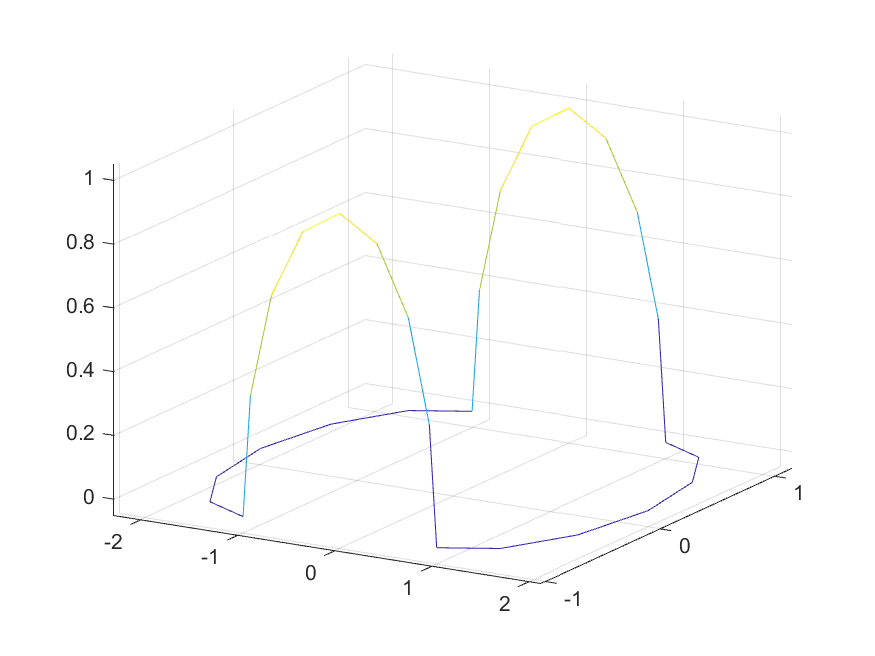
\includegraphics[width=0.4\textwidth]{ogrodje.png}
   }
   \subfigure[Kontrolni poligon
   ]{
   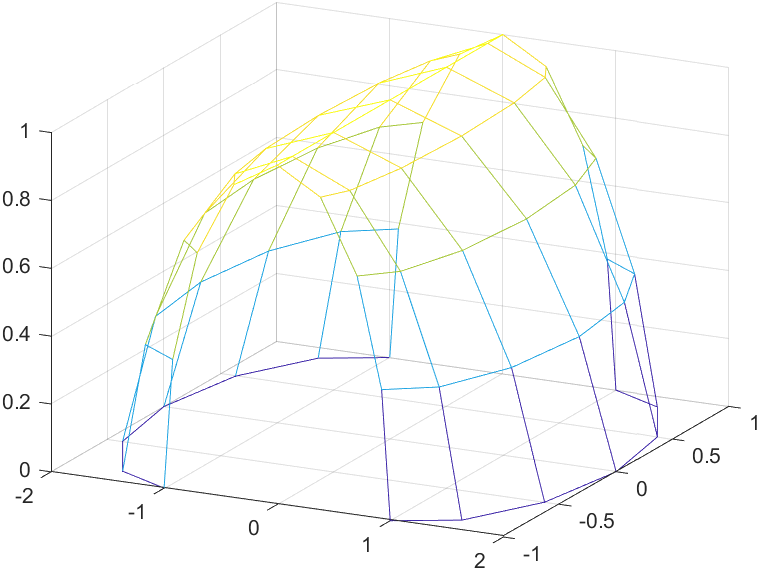
\includegraphics[width=0.4\textwidth]{dodatne_kont_t.png}
   }
   
   \subfigure[Coonsova ploskv nad kontrolnim poligonom]{
   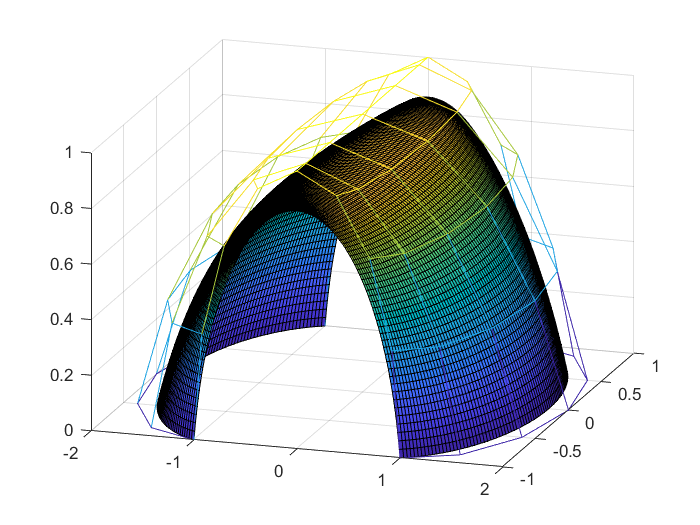
\includegraphics[width=0.35\textwidth]{primer_krivulje.png}
   }   
   \caption{Konstrukcija Coonsove ploskve}
\label{fig:whatever}
\end{figure}


\newpage




\section{Stalnost Coonsove ploskve}
\label{ch:3}

Denimo, da imamo podano Coonsova ploskev definirana nad domeno $D = [0,1]^2$. 
Izberemo si dve točki $(u_0,v_0)$ in $(u_1,v_1)$ ki razpenjata pravokotnik $R$ v domeni $D$. 
Štiri mejne krivulje pod-Coonsove ploskve definirane na $R$ se preslikajo 
v štiri krivulje na prvotni Coonsovi ploskvi. Izkaže se, da je pod-Coonsova ploskev 
definirana na $R$ enaka Coonsovi ploskvi zoženi na območje $R$. 
Oglejmo si $3 \times 3$ pod-Coonsovo ploskev
%To načelo 
%lahko uporabimo na diskretni $3 \times 3$ Coonsovi ploskivi
$$
\begin{matrix} 
   \mathbf{b}_{i-1,j-1} & \mathbf{b}_{i-1,j} & \mathbf{b}_{i-1,j+1}\\
   \mathbf{b}_{i,j-1} & \mathbf{b}_{i,j} & \mathbf{b}_{i,j+1}\\
   \mathbf{b}_{i+1,j-1} & \mathbf{b}_{i+1,j} & \mathbf{b}_{i+1,j+1}.
\end{matrix}
$$ 
V primeru da poznamo robne točke lahko notranjo točko $\mathbf{b}_{i,j}$
določimo z enačbo \eqref{diskertni}:  
\begin{align*}
   \mathbf{b}_{i,j} =& -\frac{1}{4}(\mathbf{b}_{i-1,j-1} + \mathbf{b}_{i+1,j-1} +
      \mathbf{b}_{i-1,j+1} + \mathbf{b}_{i+1,j+1}) \\
      &+\frac{1}{2}(\mathbf{b}_{i-1,j} + \mathbf{b}_{i,j-1}+
      \mathbf{b}_{i,j+1} + \mathbf{b}_{i+1,j}).\\
\end{align*}
To lahko zapišemo bolj kompaktno s pomočjo maske:
$$
\mathbf{b}_{i,j} = \frac{1}{4} \times 
\begin{matrix*}[r]
-1 && 2 && -1 \\
2 && \sbullet && 2\\
-1 && 2 && -1.
\end{matrix*}
$$
Če zgornjo masko uporabimo na vseh kontrolnih točkah 
$\mathbf{b}_{i,j},$ $i = 1,2,\dots,$ $m-1$ in $j = 1,2,\dots,n-1$
dobimo $(m-1)(n-1)$ linearnih enačb.
Ker je mreža sestavljena iz $(m+1)(n+1)$ kontrolnih točk, dane pa imamo samo robne
točke lahko ostalih $(m-1)(n-1)$ enolično določimo s pomočjo sistema
linearnih enačb. Določitev točk se tako prevede
na reševanje sistema $(m+1)(n+1)$ linearnih enačb, kjer so v sistemu robne točke že določene.

Oglejmo si $3 \times 3$ masko s splošnimi parametri, kjer se  kontrolna točka 
$\mathbf{b}_{i,j}$ izraža na sledeč način:
$$
\mathbf{b}_{i,j} =  \quad 
\begin{matrix*}[r]
\alpha && \beta && \alpha \\
\beta && \sbullet && \beta \\
\alpha && \beta && \alpha
\end{matrix*}
$$
V primeru da sta $(\alpha, \beta) = (-0.25, 0.5)$ dobimo Coonsovo
ploskev. 
Podobno kot prej ponovno rešimo sistem $(m+1)(n+1)$ linearnih enačb, a tokrat
s parametroma $\alpha$ in $\beta$.
Privzeli bomo, da velja $4\alpha + 4\beta = 1$, saj 
tako ohranjamo afinost maske. 
S perturbiranjem parametrov 
$\alpha$ in $\beta$ dobimo torej nov razred kontrolnih shem, imenujemo jih stalne 
krivulje (angl. \textit{permanence patches}). V članku \cite{DCP}  so raziskovali
vpliv $\alpha$ na optimalno oblike ploskve. Ugotovili so, da za izbrana $m$ in $n$
ni vedno ene optimalne vrednosti za $\alpha$, ki da dobro obliko ploskve.

\section{Stalne Coonsove ploskve}
\label{ch:4}

Po definiciji diskretne Coonsove ploskve je ena kontrolna točka odvisna le od osmih 
robnih in krajiščih točk, torej gre za lokalno odvisnost. V primeru ko govorimo o stalnih ploskvah 
($\alpha \neq  -0.25$), je točka odvisna od vseh mejnih točk, zato govorimo 
o globalni odvisnosti. Ta odvisnost nam potencialno lahko pripomore pri ustvarjanju 
``boljše'' krivulje.

Oglejmo si še nekaj primerov ploskev pri različnih parametrih $\alpha$ in $\beta$.
V primeru, da na sliki \ref{fig:whatever} pustimo okvir kontrolnih točk enak,
namesto parametra $\alpha =- 0.25$ pa uporabimo 
parametre $\alpha = -0.26$, $\alpha = -0.23$ ter $\alpha = 0$ in rešimo sistem
linearnih enačb dobimo krivulje prikazane na sliki \ref{fig:coons_pospl}.

\begin{figure}[ht!]
   \centering
   \subfigure[Stalna krivulja pridobljena s parametrom $\alpha = -0.26$]{
   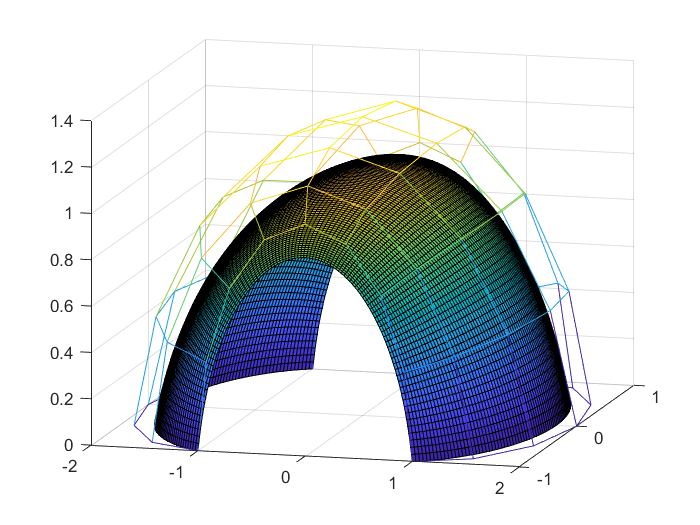
\includegraphics[width=0.4\textwidth]{square_26.png}
   }
   \subfigure[Stalna krivulja pridobljena s parametrom $\alpha = -0.23$]{
   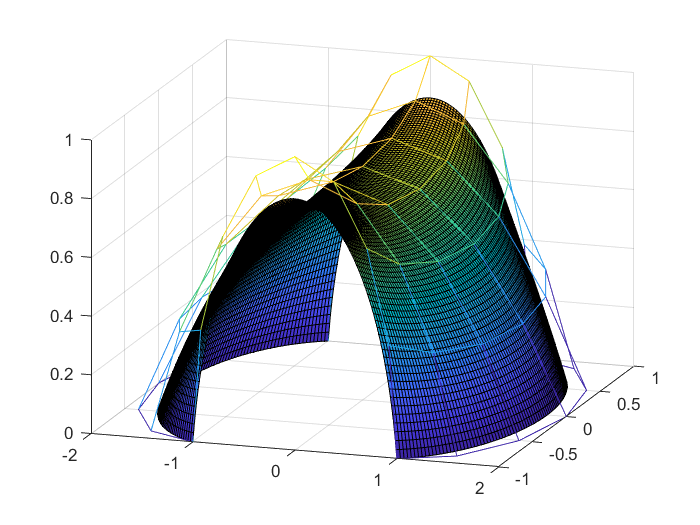
\includegraphics[width=0.4\textwidth]{square_23.png}
   }
   \subfigure[Stalna ``minimalna'' krivulja pridobljena s parametrom $\alpha = 0$]{
   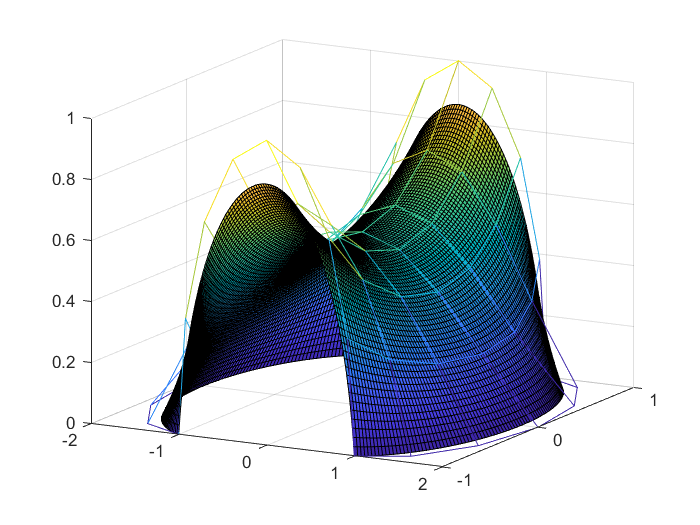
\includegraphics[width=0.4\textwidth]{square_0.png}
   }
   \caption{Stalne krivulje pridobljene z reševanjem sistemov linearnih enačb}
\label{fig:coons_pospl}
\end{figure}

Dani poligoni izhajajo iz torusnih oblik in z modifikacijo $\alpha$ lahko pridemo do želene oblike.
Kot zanimivost se izkaže da pri izbiri parametra $\alpha = 0$ in ob upoštevanju afinosti,
dobimo ploskev, katere površina je minimalna za dan okvir krivulj. To se vidi iz Laplasove parcialne 
diferencialne enačbe:
$$\mathbf{p}_{uu} + \mathbf{p}_{vv} = 0.$$

\section{Trikotne stalne Coonsove ploskve}

Oglejmo si primer, ko imamo tri robne krivulje definirane nad trikotnikom 
namesto štirih robnih krivulj nad pravokotnikom.
Pojavi se naslednje vprašanje, če imamo podane tri robne kontrolne poligone 
ki razpenjajo zunanjost trikotnika, ali obstaja  ``dobra''
kontrolna mreža, ki zapolni omejeno območje. 
Podobno kot v razdelkih \ref{ch:3} in \ref{ch:4} lahko uporabimo načelo 
stalnosti za masko:
$$
\mathbf{b}_{\mathbf{i}} =  \quad 
\begin{matrix*}[r]
          &       &       & \alpha   &       &       & \\
          &       & \beta &          & \beta &       & \\
          &         \beta &       & \sbullet &       & \beta & \\
   \alpha &       & \beta &          & \beta &       & \alpha,
\end{matrix*}
$$
kjer zaradi pogoja afinosti ponovno zahtevamo, da je $3\alpha + 6\beta = 1$.

Načelo stalosti uporabimo za vse $\mathbf{b}_{\mathbf{i}}$, kjer je $\mathbf{i} >0$,
robne točke pa so že podane. 
Podobno kot prej rešimo sistem z $\binom{m+1}{2}$ linearnih enačb, 
kjer je $m$ število kontrolnih točk na eni stranici trikotnika.
Robne točke v sistemu so ponovno že določene.

Ponovno pri parametru $\alpha = 0$ dobimo ploskev, 
katere površina je minimalna za dan okvir krivulj, kar se ponovno vidi iz 
Laplasove parcialne diferencialne enačbe.
Na sliki \ref{fig:trikotne} vidimo tri možne oblike stalne trikotne
krpe s parametri $\alpha = 0,$ $\alpha = -1/9$ ter $\alpha = -1/6$.
\begin{figure}[ht!]
   \centering
   \subfigure[Stalna trikotna krpa pridobljena s parametrom $\alpha = -1/6$]{
   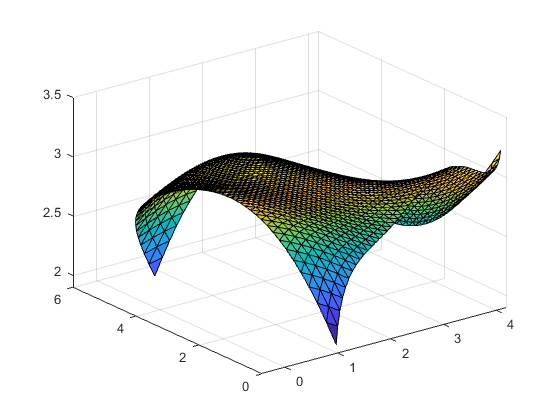
\includegraphics[width=0.45\textwidth]{trikotne_1_6.png}
   }
   \subfigure[Stalna trikotna krpa pridobljena s parametrom $\alpha = -1/9$]{
   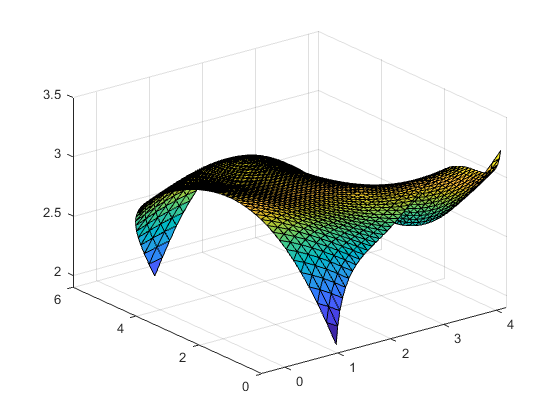
\includegraphics[width=0.45\textwidth]{trikotne_1_9.png}
   }
   
   \subfigure[Stalna ``minimalna'' trikotna krpa pridobljene s parametrom $\alpha = 0$]{
   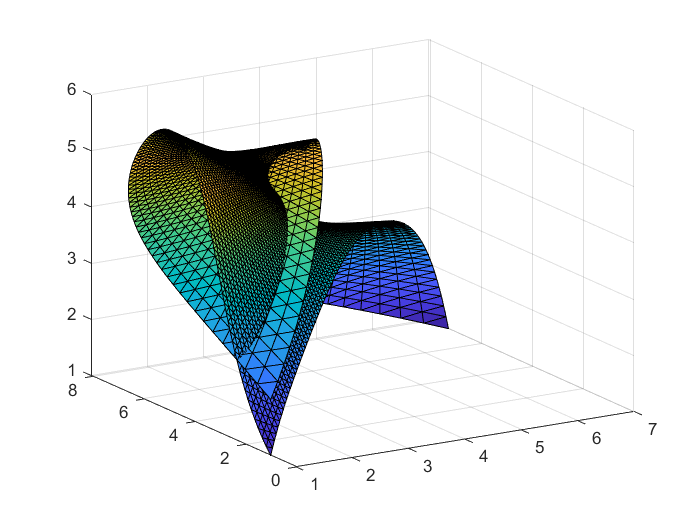
\includegraphics[width=0.5\textwidth]{trikotne_0.png}
   }   
   \caption{Stalne trikotne krpe pridobljene z reševanjem sistemov enačb.}
\label{fig:trikotne}
\end{figure}

\section{Zaključek}

V seminarski nalogi smo konstruirali diskretne Coonsove ploskve in jih posplošili na stalne
ploskve, tako za ploske definirane nad pravokotnikom kot za ploskve definirane nad 
trikotnikom. Posplošitev nam je omogočala
izdelavo oblik, ki so bolj zaželene od standardnih Coonsovih oblik. Ogledali smo 
si vpliv parametrov stalnih ploskev in jih grafično prikazali.

\newpage

\begin{thebibliography}{99}
   \bibitem{DCP}
   G.~Farin, F.~Hansford, \emph{Discrete Coons patches}, 
   \bibitem{GR}
   J.~Grošelj \url{https://users.fmf.uni-lj.si/groseljj/mat-rpgo/2022-2023/rpgo_zbirka_nalog.pdf#naloga12}
\end{thebibliography}
\end{document}